\documentclass{beamer}
\usetheme{Warsaw}

\usepackage[utf8]{inputenc}
\usepackage{german}
\usepackage{mathtools}
\usepackage{listings}
\usepackage{tikz}
\usetikzlibrary{shapes}

\tikzset{onslide/.code args={<#1>#2}{\only<#1>{\pgfkeysalso{#2}}}}

\title[Quadtrees]
{Programmierkonzepte und Algorithmen: Quad-/Octrees}
\useoutertheme{infolines}
\subtitle{Spatiale Suche und Kollisionserkennung}
\author[Moukayed, Kinder]
{Fadi Moukayed (539502) \\ Eugen Kinder (539723)}
\date[ProgKo WS2016/17]
{ProgKo WS2016/17 -- HTW Berlin AI(M)}
\subject{Computer Science}

\begin{document}
  
\frame{\titlepage}
\begin{frame}
  \frametitle{Inhalte}
  \tableofcontents
\end{frame}

\section{Problematik}

\begin{frame}
  \frametitle{Spieleprogrammierung}
  \framesubtitle{Fast real-time collision detection -- TheDigitalSorceress/YouTube}
  \begin{center}
    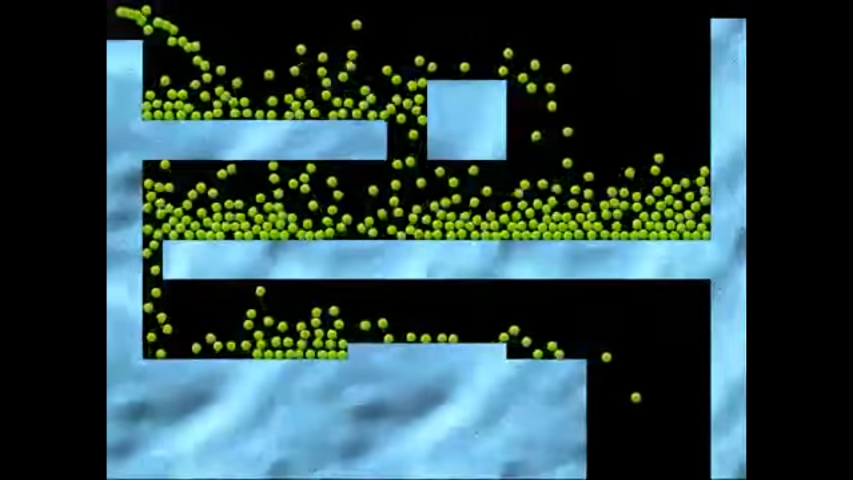
\includegraphics[scale=0.5]{rsrc/greencirc}
    
    \tiny \it Fast real-time collision detection -- TheDigitalSorceress/YouTube
  \end{center}
\end{frame}

\begin{frame}
  \frametitle{Spieleprogrammierung}
  \framesubtitle{Touhou 15 LoLK: Legacy of the Luncatic Kingdom (2015)}
  \begin{center}
    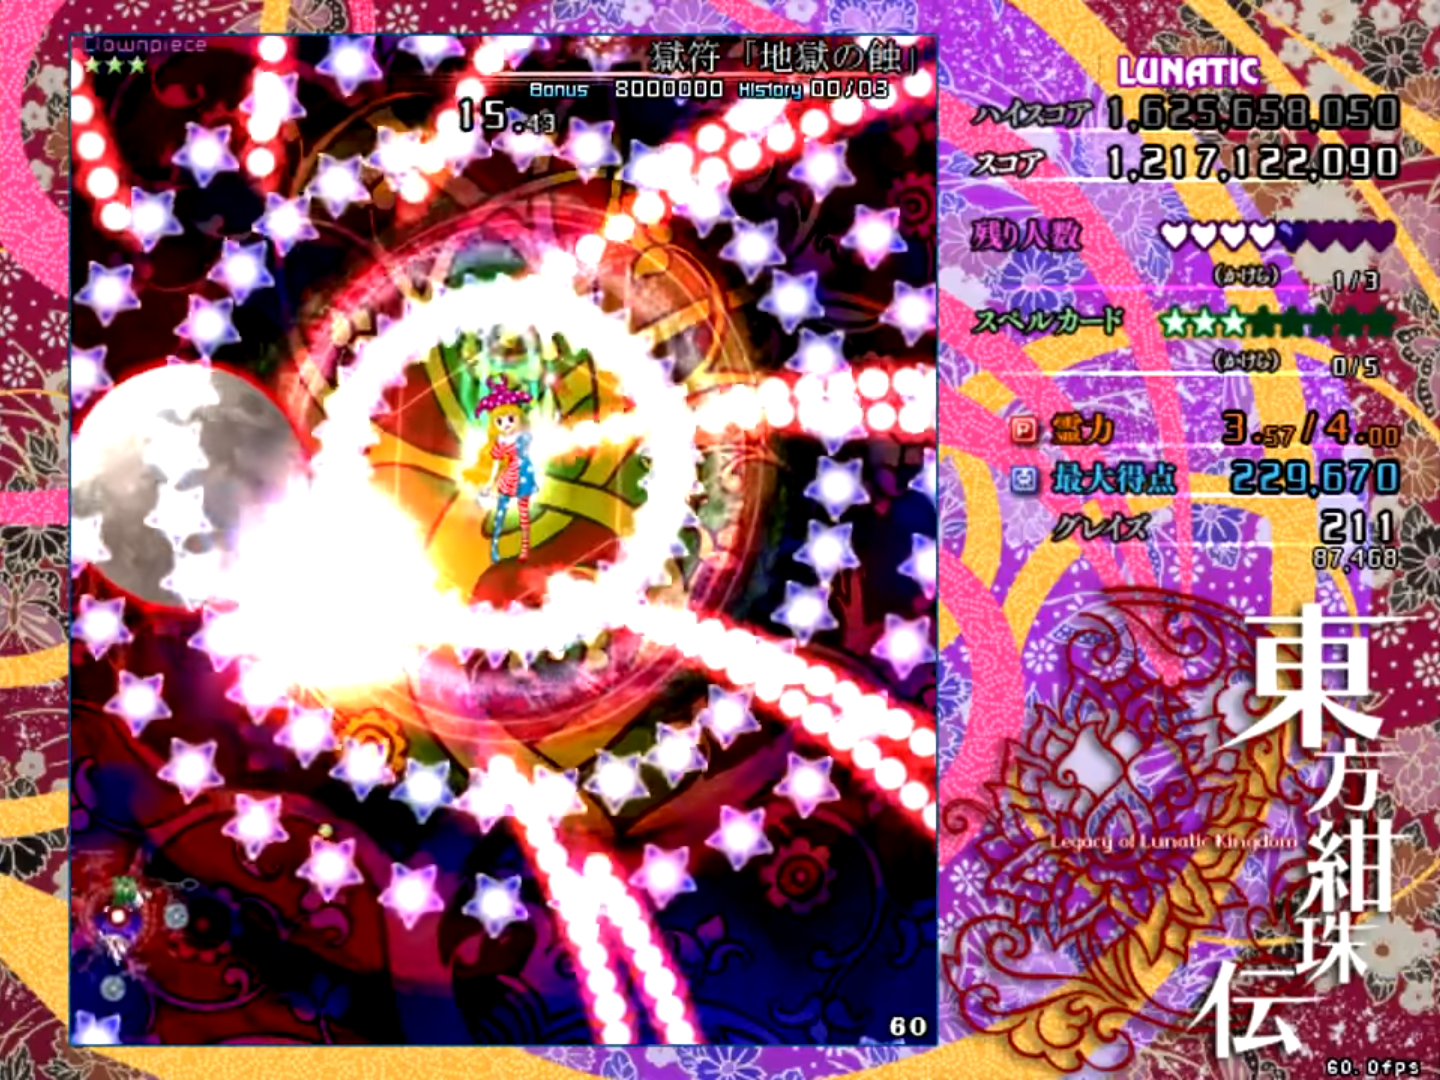
\includegraphics[scale=0.20]{rsrc/touhou}
    
    \tiny \it Touhou 15 LoLK: Legacy of the Luncatic Kingdom (2015)
  \end{center}
\end{frame}

\begin{frame}
  \frametitle{Spieleprogrammierung}
  \framesubtitle{Touhou 15 LoLK: Legacy of the Luncatic Kingdom (2015) - Bounding Boxes}
  \begin{figure}
    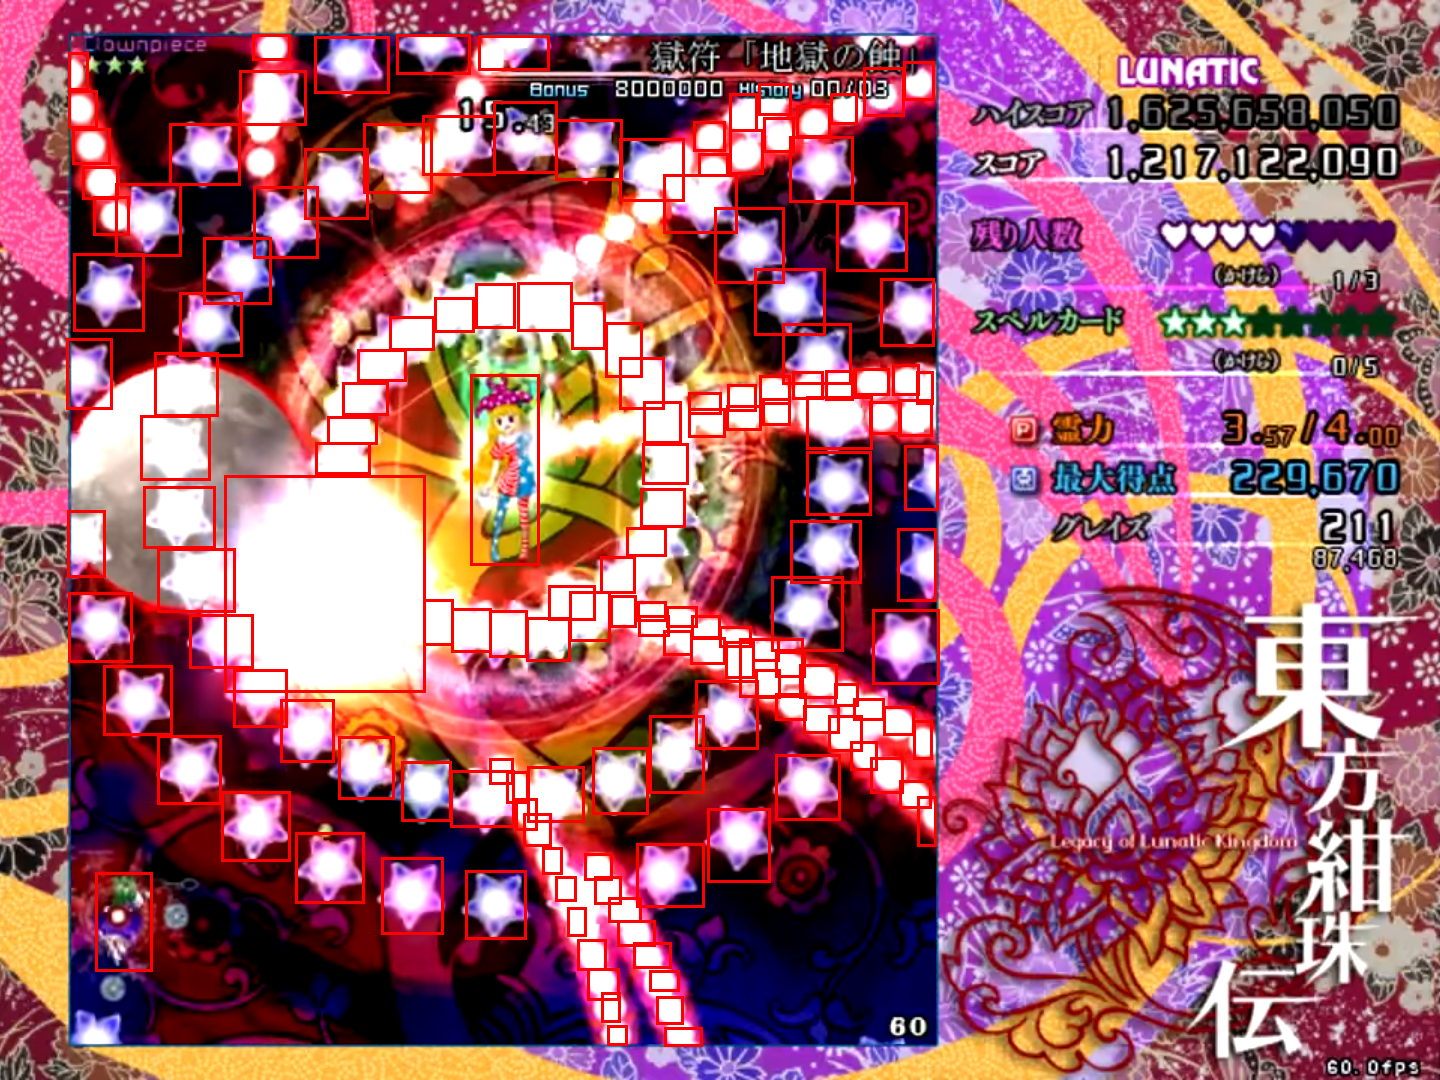
\includegraphics[scale=0.25]{rsrc/touhoubbox}
  \end{figure}
\end{frame}

\section{Grundlagen}

\begin{frame}
  \frametitle{Grundlagen}
  \framesubtitle{Bounding Boxes - Geometrie}
  \begin{figure}
    \begin{tikzpicture}
      \draw (-0.25,-0.25) node {$x,y$};
      \draw (4.25,1) node {$h$};
      \draw (2,2.25) node {$w$};
      \draw (0,0) rectangle (4,2);
    \end{tikzpicture}
  \end{figure}
  
  \begin{block}{Def. Quadrat}
    \begin{itemize}
      \item $(x,y,w,h) \in \mathbb{R}^4$
      \begin{itemize}
        \item $x, y \in \mathbb{R}$
        \item $w \in \mathbb{R}$ (En.: Width / Breite)
        \item $h \in \mathbb{R}$ (En.: Height / Höhe)
      \end{itemize}
    \end{itemize}
  \end{block}
\end{frame}

\begin{frame}
  \frametitle{Grundlagen}
  \framesubtitle{Bounding Boxes - Überschneidung}
  \begin{figure}
    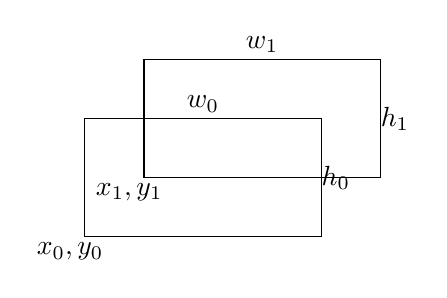
\begin{tikzpicture}[scale=0.75]
      \draw (-0.25,-0.25) node {$x_0,y_0$};
      \draw (4.25,1) node {$h_0$};
      \draw (2,2.25) node {$w_0$};
      \draw (0,0) rectangle (4,2);
      
      \draw (0.75,0.75) node {$x_1,y_1$};
      \draw (5.25,2) node {$h_1$};
      \draw (3,3.25) node {$w_1$};
      \draw (1,1) rectangle (5,3);
    \end{tikzpicture}
  \end{figure}
  
  \begin{block}{Def. Intersect}
      \small
      $intersect:\mathbb{R}^4 \times \mathbb{R}^4 \rightarrow \mathbb{B}$
      \begin{flalign*}
          (x_0,y_0,w_0,h_0),(x_1,y_1,w_1,h_1) \mapsto 
          (x_0 + w_0 \geq x_1) &\wedge (y_0 + h_0 \geq y_1)~\wedge \\
          (x_0 \leq x_1 + w_1) &\wedge (y_0 \leq y_1 + h_1) 
      \end{flalign*}
  \end{block}
\end{frame}

\begin{frame}
  \frametitle{Naive Kollisionserkennung}
  \framesubtitle{Komplexität}
  \begin{itemize}
    \item Menge der Objekte $O = \{o_1,o_2,...,o_n\}$
    \begin{itemize}
      \item $O \subseteq \mathbb{R}^4$
      \item $|O| = n$
    \end{itemize}
    
    \item Für $o_1$
    \begin{itemize}
      \item $intersect(o_1,o_2) \vee intersect(o_1,o_3) \vee ... \vee intersect(o_1,o_n)$
      \item $(n - 1)$ intersect-Operationen
    \end{itemize}
    
    \item Für alle Objekte in $O$
    \begin{itemize}
      \item $n(n-1)$ intersect-Operationen
    \end{itemize}
  \end{itemize}
\end{frame}

\begin{frame}
  \frametitle{Naive Kollisionserkennung}
  \framesubtitle{Komplexität}
  \begin{columns}
    \column{0.38\linewidth}
      \begin{itemize}
        \item Naive Kollisionserkennung
        \begin{itemize}
          \item Komplexität pro Objekt: $O(n)$
          \item Komplexität für alle Objekte: $O(n^2)$
        \end{itemize}
      \end{itemize}
    \column{0.58\linewidth}
      \begin{center}
        
\includegraphics[scale=0.75]{rsrc/facepalm}
        
        \tiny \it Picard Facepalm, Deja Q: Star Trek TNG
      \end{center}
  \end{columns}
\end{frame}

\begin{frame}
  \frametitle{Naive Kollisionserkennung}
  \framesubtitle{Komplexität}
  \begin{columns}
    \column{0.38\linewidth}
      \begin{itemize}
        \item Es gibt alternativen
        \item Trees!
      \end{itemize}
    \column{0.58\linewidth}
      \begin{center}
        
\includegraphics[scale=0.40]{rsrc/picardyeah}
        
        \tiny \it J~.L. Picard: Star Trek TNG
      \end{center}
  \end{columns}
\end{frame}

\begin{frame}
  \frametitle{Bäume}
  \framesubtitle{Recap}
  \begin{center}
    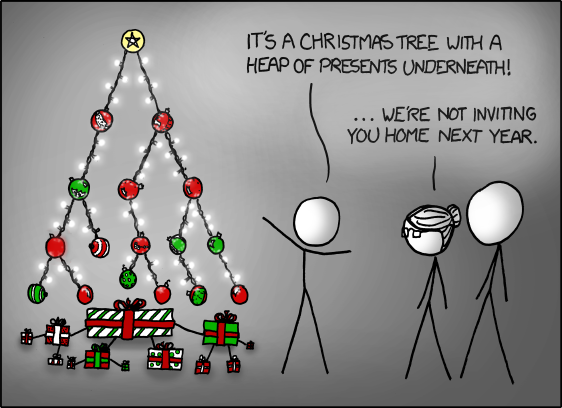
\includegraphics[scale=0.5]{rsrc/tree_xkcd835}
    
    \tiny \it XKCD \#835: Tree
  \end{center}
\end{frame}

\begin{frame}
  \frametitle{Bäume}
  \framesubtitle{Recap}
  \begin{itemize}
    \item Baum: Spezieller Typ von Graph
    \begin{itemize}
      \item Zusammenhängend (Keine Waisenknoten)
      \item Zyklusfrei
      \item Ungerichtet
    \end{itemize}
  \end{itemize}
\end{frame}

\begin{frame}
  \frametitle{Bäume}
  \framesubtitle{Binär}
  \begin{figure}
    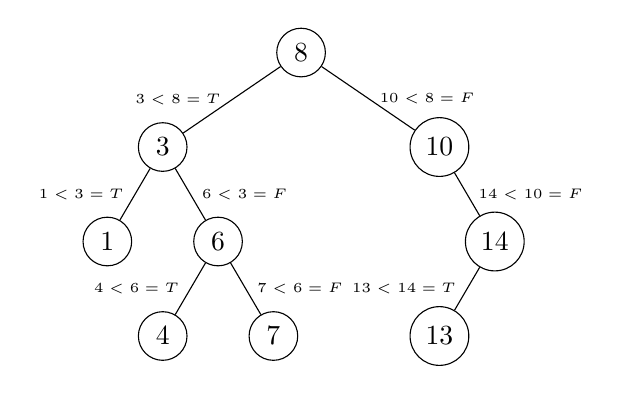
\begin{tikzpicture}[
        level distance=12mm, 
        level 1/.style={sibling distance=10em},
        level 2/.style={sibling distance=4em},
        every node/.style = {shape=circle, draw}]
      \node {8}
        child {node {3}
          child {node {1}
            edge from parent node[left, draw=none] {\tiny $1 < 3 = T$}}
          child {node {6}
            child {node {4}
              edge from parent node [left, draw=none] {\tiny $4 < 6 = T$}}
            child {node {7}
              edge from parent node [right, draw=none] {\tiny $7 < 6 = F$}}
          edge from parent node[right, draw=none] {\tiny $6 < 3 = F$}}
          edge from parent node[left, draw=none] {\tiny $3 < 8 = T$}}
        child {node {10}
          child[style={edge from parent/.style={draw=none}}] {node[draw=none] {}}
          child {node {14}
            child {node {13}
              edge from parent node[left, draw=none] {\tiny $13 < 14 = T$}}
            child[style={edge from parent/.style={draw=none}}] {node[draw=none] {}}
          edge from parent node [right, draw=none] {\tiny {$14 < 10 = F$}}}
          edge from parent node [right, draw=none] {\tiny $10 < 8 = F$}};
    \end{tikzpicture}
  \end{figure}
  \begin{itemize}
    \item Binary Search Tree (BST)
    \begin{itemize}
      \item Binäre Ordnungsrelation "`$<$"'
      \item $<:\mathbb{R} \times \mathbb{R} \rightarrow \mathbb{B}$
    \end{itemize}
  \end{itemize}
\end{frame}

\begin{frame}
  \frametitle{Bäume}
  \framesubtitle{Ternär}
  \begin{center}
    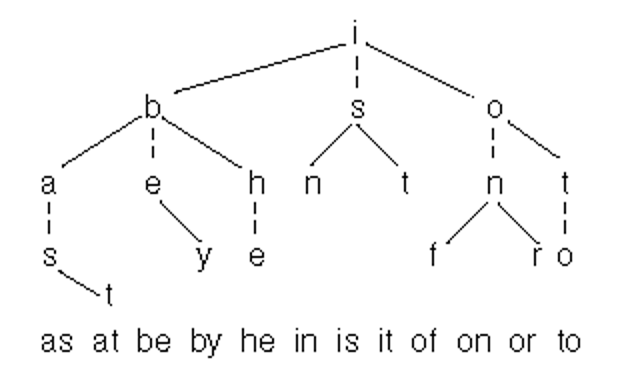
\includegraphics[scale=0.5]{rsrc/tst}
    
    \tiny \it Ternary search tree for 12 words, J. Bentley, B. Sedgewick, Dr. Dobbs (1998)
  \end{center}
  \begin{itemize}
    \item Ternary Search Tree (TST)
    \begin{itemize}
      \item Ternäre Ordnungsrelation $cmp$
      \item $cmp:\Sigma \times \Sigma \rightarrow \{lo,eq,hi\}$
    \end{itemize}
  \end{itemize}
\end{frame}

\section{Quaternärbaume}

\begin{frame}
  \frametitle{Bäume}
  \framesubtitle{Quaternär}
  \begin{itemize}
    \item Quaternärbaum
    \item Quaternäre Ordnungsrelation
    \item $?:? \times ? \rightarrow Y$
    \begin{itemize}
      \item $|Y| = 4$
    \end{itemize}
  \end{itemize}
\end{frame}

\begin{frame}
  \frametitle{Quaternärbaume}
  \framesubtitle{Konzept}
  \begin{figure}
    \begin{tikzpicture}
      \draw (0,0) rectangle (8,5);
      \only<2->{\draw (0,2.5) -- (8,2.5)};
      \only<2->{\draw (4,0) -- (4,5)};
      \only<3-4>{\draw (6,3.75) node {I}};
      \only<3-4>{\draw (2,3.75) node {II}};
      \only<3-4>{\draw (2,1.25) node {III}};
      \only<3-4>{\draw (6,1.25) node {IV}};
      \only<5->{\draw (6,3.75) node {NE}};
      \only<5->{\draw (2,3.75) node {NW}};
      \only<5->{\draw (2,1.25) node {SW}};
      \only<5->{\draw (6,1.25) node {SE}};
      \only<4->{
        \draw (0,0) node[left] {\tiny $x,y$};
        \draw (0,2.5) node[left] {\tiny $x,y+\frac{1}{2}h$};
        \draw (0,5) node[left] {\tiny $x,y+h$};
        \draw (4,5.25) node {\tiny $x+\frac{1}{2}w,y+h$};
        \draw (8,5) node[right] {\tiny $x+w,y+h$};
        \draw (8,2.5) node[right] {\tiny $x+w,y+\frac{1}{2}h$};
        \draw (8,0) node[right] {\tiny $x+w,y$};
        \draw (4,0) node[below] {\tiny $x+\frac{1}{2}w,y$}};
    \end{tikzpicture}
  \end{figure}
\end{frame}

\begin{frame}
  \frametitle{Quaternärbaume}
  \framesubtitle{Datenstruktur}
  \begin{figure}
    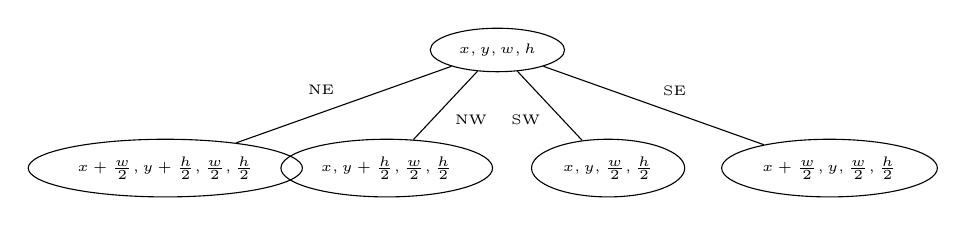
\begin{tikzpicture}[
      level 1/.style={sibling distance=8em},
      every node/.style={shape=ellipse, draw}]
      \node {\tiny $x,y,w,h$}
        child {node {\tiny $x+\frac{w}{2},y+\frac{h}{2},\frac{w}{2},\frac{h}{2}$}
          edge from parent node[above left, draw=none] {\tiny NE}}
        child {node {\tiny $x,y+\frac{h}{2},\frac{w}{2},\frac{h}{2}$}
          edge from parent node [below right, draw=none] {\tiny NW}}
        child {node {\tiny $x,y,\frac{w}{2},\frac{h}{2}$}
          edge from parent node [below left, draw=none] {\tiny SW}}
        child {node {\tiny $x+\frac{w}{2},y,\frac{w}{2},\frac{h}{2}$}
          edge from parent node [above right, draw=none] {\tiny SE}};
    \end{tikzpicture}
  \end{figure}
  \begin{itemize}
    \item Quaternäre Ordnungsrelation
    \item $quadrant:\mathbb{R}^4 \times \mathbb{R}^4 \rightarrow \{NE,NW,SW,SE\}$
  \end{itemize}
\end{frame}
  
\begin{frame}[fragile]
  \frametitle{Quaternärbaume}
  \framesubtitle{Datenstruktur}
  \begin{figure}
    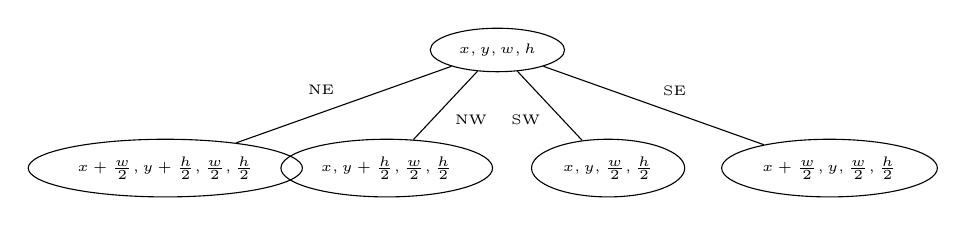
\begin{tikzpicture}[
      level 1/.style={sibling distance=8em},
      every node/.style={shape=ellipse, draw}]
      \node {\tiny $x,y,w,h$}
        child {node {\tiny $x+\frac{w}{2},y+\frac{h}{2},\frac{w}{2},\frac{h}{2}$}
          edge from parent node[above left, draw=none] {\tiny NE}}
        child {node {\tiny $x,y+\frac{h}{2},\frac{w}{2},\frac{h}{2}$}
          edge from parent node [below right, draw=none] {\tiny NW}}
        child {node {\tiny $x,y,\frac{w}{2},\frac{h}{2}$}
          edge from parent node [below left, draw=none] {\tiny SW}}
        child {node {\tiny $x+\frac{w}{2},y,\frac{w}{2},\frac{h}{2}$}
          edge from parent node [above right, draw=none] {\tiny SE}};
    \end{tikzpicture}
  \end{figure}
  \begin{lstlisting}[language=C++,basicstyle={\small}]
    template <typename T> struct node {
      std::vector<T> elements;
      double x, y, w, h;
      std::array<std::unique_ptr<node>, 4> children;
    };
  \end{lstlisting}
\end{frame}

\section{Algorithmen}

\begin{frame}
  \frametitle{Quaternärbaume}
  \framesubtitle{Algorithmen - Subdivision}
  \begin{figure}
    \begin{tikzpicture}[
      grow=right,
      level distance=50mm,
      sibling distance=10mm,
      every node/.style={shape=ellipse, draw}]
      \only<1>{\node {\tiny $K(x,y,w,h)$}};
      \only<2->{
        \node {\tiny $K(x,y,w,h)$}
        child {node {\tiny $K_{NE}(x+\frac{w}{2},y+\frac{h}{2},\frac{w}{2},\frac{h}{2}$)} edge from parent[onslide=<1-2>{draw=none}]}
        child {node {\tiny $K_{NW}(x,y+\frac{h}{2},\frac{w}{2},\frac{h}{2})$} edge from parent[onslide=<2>{draw=none}]}
        child {node {\tiny $K_{SW}(x,y,\frac{w}{2},\frac{h}{2})$} edge from parent[onslide=<2>{draw=none}]}
        child {node {\tiny $K_{SE}(x+\frac{w}{2},y,\frac{w}{2},\frac{h}{2})$} edge from parent[onslide=<2>{draw=none}]}};
    \end{tikzpicture}
  \end{figure}
  \begin{enumerate}
    \item Vaterknoten $K$ auswählen
    \pause
    \item Vier Knoten $K_{NE}, K_{NW}, K_{SE}, K_{SW}$ erzeugen
    \pause
    \item $K_{NE}, K_{NW}, K_{SE}, K_{SW}$ als Kindknoten von $K$ hinzufügen
  \end{enumerate}
\end{frame}

\begin{frame}
  \frametitle{Quaternärbaume}
  \framesubtitle{Algorithmen - Optimal Fit}
  \begin{itemize}
    \item Optimal Fit: Suche den (räumlich) kleinsten Knoten, welches ein gegebenes Quadrat $Q = (x,y,w,h)$ umschließt
    \item Input: Wurzelknoten, $Q$
    \item Output: Knoten $K$
    \item Nachbedingung: $contains(K,Q) = T$
  \end{itemize}
  \begin{block}{Def. $contains$}
    \small
    $contains:\mathbb{R}^4 \times \mathbb{R}^4 \rightarrow \mathbb{B}$
    \begin{flalign*}
      (x_0,y_0,w_0,h_0),(x_1,y_1,w_1,h_1) \mapsto 
      &(x_1 \geq x_0)~\wedge \\
      &(y_1 \geq y_0)~\wedge \\
      &(x_1 + w_1 \leq x_0 + w_0)~\wedge \\
      &(y_1 + h_1 \leq y_0 + h_0) 
    \end{flalign*}
  \end{block}
\end{frame}

\begin{frame}[fragile]
  \frametitle{Quaternärbaume}
  \framesubtitle{Algorithmen - Optimal Fit}
  \begin{block}{Optimal-Fit Pseudocode}
    \begin{lstlisting}[language=Python,basicstyle={\small}]
    def optimalfit(K, Q):
        if contains(K, Q):
            if leaf(K):
                return K
            else:
                for child in (K.ne, K.nw, K.sw, K.se):
                    if contains(child, Q):
                        return optimalfit(child, Q)
                return K
        else:
            return None
    \end{lstlisting}
  \end{block}
\end{frame}

\begin{frame}
  \frametitle{Quaternärbaume}
  \framesubtitle{Algorithmen - Optimal Fit}
  \begin{figure}
    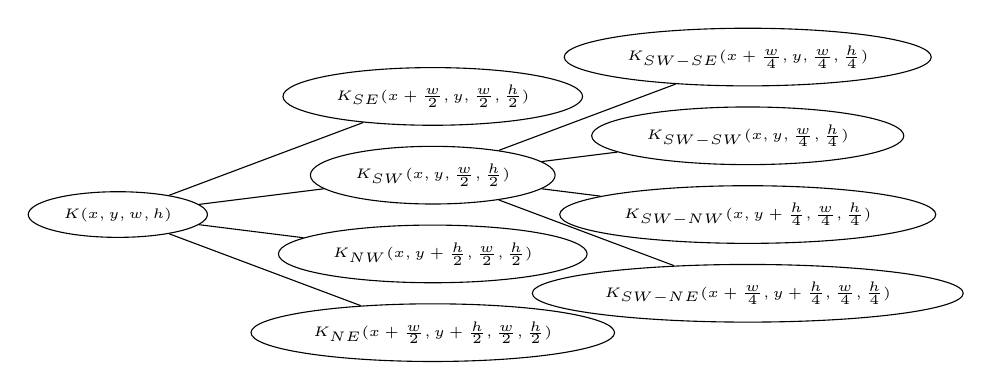
\begin{tikzpicture}[
      grow=right,
      level distance=40mm,
      sibling distance=10mm,
      every node/.style={shape=ellipse, draw}]
      \node {\tiny $K(x,y,w,h)$}
        child {node {\tiny $K_{NE}(x+\frac{w}{2},y+\frac{h}{2},\frac{w}{2},\frac{h}{2})$}}
        child {node {\tiny $K_{NW}(x,y+\frac{h}{2},\frac{w}{2},\frac{h}{2})$}}
        child {node[onslide=<3->{fill=black,text=white}] {\tiny $K_{SW}(x,y,\frac{w}{2},\frac{h}{2})$}
          child {node {\tiny $K_{SW-NE}(x+\frac{w}{4},y+\frac{h}{4},\frac{w}{4},\frac{h}{4})$}}
          child {node {\tiny $K_{SW-NW}(x,y+\frac{h}{4},\frac{w}{4},\frac{h}{4})$}}
          child {node[onslide=<5>{fill=black},onslide=<6->{fill=blue},onslide=<5->{text=white}] {\tiny $K_{SW-SW}(x,y,\frac{w}{4},\frac{h}{4})$}}
          child {node[onslide=<4->{fill=black,text=white}] {\tiny $K_{SW-SE}(x+\frac{w}{4},y,\frac{w}{4},\frac{h}{4})$}}}
        child {node[onslide=<2->{fill=black,text=white}] {\tiny $K_{SE}(x+\frac{w}{2},y,\frac{w}{2},\frac{h}{2})$}};
    \end{tikzpicture}
  \end{figure}
  \begin{itemize}
    \item Gesucht: $Q = (x,y,\frac{w}{8},\frac{h}{8})$
    \only<2>{\item $contains(K_{SE},Q) = F$}
    \only<3>{\item $contains(K_{SW},Q) = T$
      \begin{itemize}
        \item Wende den Optimal-Fit-Algorithmus an mit $(K_{SW},Q)$
      \end{itemize}}
    \only<4>{\item $contains(K_{SW-SE},Q) = F$}
    \only<5>{
      \item $contains(K_{SW-SW},Q) = T$
      \begin{itemize}
        \item Wende den Optimal-Fit-Algorithmus an mit $(K_{SW-SW},Q)$
      \end{itemize}}
    \only<6>{\item $K_{SW-SW}$ ist ein Blatt $\rightarrow$ abbruch mit Ergebnis $K_{SW-SW}$}
  \end{itemize}
\end{frame}

\begin{frame}
  \frametitle{Quaternärbaume}
  \framesubtitle{Algorithmen - Insert}
  \begin{itemize}
    \item Der Einfüge-Algorithmus Setzt sich aus aus $optimalfit$ + $subdivide$
    \item Input: Knoten $K$, Quadratförmiges Element $E$, Schellwert $N$
    \item Ablauf von $insert(K,E)$
    \begin{itemize}
      \item Rufe $optimalfit(K,E)$ auf, speichere Ergebnis in $O$
      \item Füge E in die Elementliste von O ein
      \item Wenn die Elementliste von O mindestens N elemente enthält
      \begin{itemize}
        \item Wende $subdivide$ auf O an
        \item Entferne alle Elemente aus Elementliste von O und füge alle in O neu ein
      \end{itemize}
    \end{itemize}
  \end{itemize}
\end{frame}

\begin{frame}
  \frametitle{Quaternärbaume}
  \framesubtitle{Algorithmen - Demonstration}
  \begin{center}
    Demonstration \\
    \hfill\break
    http://github.com/kochab/tclquadtree
  \end{center}
\end{frame}

\begin{frame}
  \frametitle{Quaternärbaume}
  \framesubtitle{Kollisionserkennung}
  \begin{itemize}
    \item Verwendung von Quadtrees zur Kollisionserkennung
    \item Input: Knoten $K$, Quadratförmiges Element $E$
    \item Verfahren
    \begin{itemize}
      \item Rufe $optimalfit(K, E)$ auf, speichere Ergebnis in $O$
      \item Für alle Elemente $X$ die in den Knoten des Pfades $O - ROOT$ enthalten sind
      \begin{itemize}
        \item Prüfe auf Überschneidung (Kollision) mit $intersect(X,E)$
      \end{itemize}
    \end{itemize}
  \end{itemize}
\end{frame}

\begin{frame}
  \frametitle{Quaternärbaume}
  \framesubtitle{Kollisionserkennung - Beispiel}
  \centering
  \begin{figure}
    \begin{tikzpicture}[every node/.style={inner sep=0pt, shape=rectangle, draw}]]
      \only<4->{\draw[fill=gray] (5,2.5) rectangle (6,3.125)};
      \only<6->{\draw[fill=gray] (4,2.5) rectangle (6,3.75)};
      \only<7->{\draw[fill=gray] (4,2.5) rectangle (8,5)};
      \only<8->{\draw[fill=gray] (0,0) rectangle (8,5)};
      \draw (0,0) rectangle (8,5);
      \draw (0,2.5) -- (8,2.5);
      \draw (4,0) -- (4,5);
      \draw (4,3.75) -- (8,3.75);
      \draw (6,2.5) -- (6,5);
      \draw (4,3.125) -- (6,3.125);
      \draw (5,2.5) -- (5,3.75);
      \only<1>{\draw (5.125,2.85) node[fill=black,text=white] {\tiny a}};
      \only<2->{\draw (5.125,2.85) node[draw=none,fill=red,text=white] {\tiny a}};
      \only<1-4>{
        \draw (5.35,2.75) node[fill=black,text=white] {\tiny b};
        \draw (5.125,2.74) node[fill=black,text=white] {\tiny c}};
      \only<5->{
        \draw (5.35,2.75) node[draw=none,fill=red,text=white] {\tiny b};
        \draw (5.125,2.74) node[draw=none,fill=red,text=white] {\tiny c}};
      \draw (4.5,1.75) node[fill=black,text=white] {\tiny d};
      \draw (4.6,2.75) node[fill=black,text=white] {\tiny e};
      \draw (4.8,1.25) node[fill=black,text=white] {\tiny f};
      \draw (5.1,1.45) node[fill=black,text=white] {\tiny g};
      \draw (3.25,0.45) node[fill=black,text=white] {\tiny h};
      \draw (2.55,1.15) node[fill=black,text=white] {\tiny i};
      \draw (1.95,0.15) node[fill=black,text=white] {\tiny j};
      \draw (2.95,4.75) node[fill=black,text=white] {\tiny k};
      \draw (1.95,3.75) node[fill=black,text=white] {\tiny l};
      \draw (6.95,4.575) node[fill=black,text=white] {\tiny m};
      \draw (7.85,3.525) node[fill=black,text=white] {\tiny n};
      \draw (6.285,4.625) node[fill=black,text=white] {\tiny o};
      \draw (6.285,3.425) node[fill=black,text=white] {\tiny p};
      \draw (6.585,3.125) node[fill=black,text=white] {\tiny q};
      \draw (4.585,3.225) node[fill=black,text=white] {\tiny r};
      \draw (4.685,3.425) node[fill=black,text=white] {\tiny s};
      \draw (4.985,3.925) node[fill=black,text=white] {\tiny t};
      \draw (5.345,4.325) node[fill=black,text=white] {\tiny u};
      \draw (5.315,4.625) node[fill=black,text=white] {\tiny v};
      \draw (5.315,3.325) node[fill=black,text=white] {\tiny w};
      \draw (5.415,3.465) node[fill=black,text=white] {\tiny x};
      \draw (5.415,3.465) node[fill=black,text=white] {\tiny y};
      \draw (2.415,3.465) node[fill=black,text=white] {\tiny z};
    \end{tikzpicture}
  \end{figure}
  
  \only<2->{Kollisionskandidatensuche für \emph{a} (Rot)}
  
  \only<3>{$optimalfit(K,a)$}
  \only<4>{$optimalfit(K,a) = K_{NE-SW-SE}$ (\emph{Grau})}
  \only<5>{Objektlistenelemente von $K_{NE-SW-SE}$: $\{c,b\}$ als Kollisionskandidaten selektieren}
  \only<6>{Objektlistenelemente von $K_{NE-SW}$: $\emptyset$  als Kollisionskandidaten selektieren}
  \only<7>{Objektlistenelemente von $K_{NE}$: $\emptyset$  als Kollisionskandidaten selektieren}
  \only<8>{Objektlistenelemente von $K$: $\emptyset$  als Kollisionskandidaten selektieren}
  \only<9>{Ergebnis: \emph{a} hat die Kollisionskandidaten $\{c,b\}$}
  \only<10>{Zu evaluieren ist nur $intersect(a,c) \vee intersect(a,b)$}
\end{frame}

\section{Octrees}

\begin{frame}
  \frametitle{Octrees}
  \framesubtitle{Struktur}
  \begin{itemize}
    \item Quadtrees sind für Flächen (2D)
    \item Octrees sind für Räume (3D)
    \item Konzeptuell sehr ähnlich
  \end{itemize}
\end{frame}

\begin{frame}
  \frametitle{Octrees}
  \framesubtitle{Struktur}
  \begin{center}
    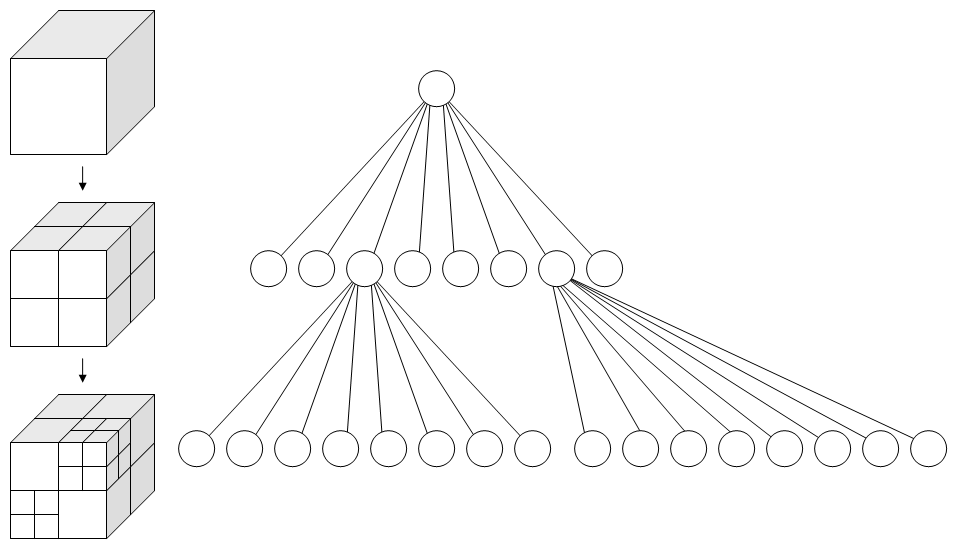
\includegraphics[scale=0.4]{rsrc/wpoctree}
    
    \tiny \it Octree - Nü, Wikimedia (License: GFDL)
  \end{center}
\end{frame}

\begin{frame}
  \frametitle{Octrees}
  \framesubtitle{Struktur}
  \begin{itemize}
    \item Subdivision in 8 Subquader
    \item Quader beschrieben durch $(x,y,z,w,h,d) \in \mathbb{R}^6$
    \begin{itemize}
      \item $d: depth$
    \end{itemize}
    \item ${contains}_{3D}: \mathbb{R}^6 \times \mathbb{R}^6 \rightarrow \mathbb{B}$
    \item ${intersect}_{3D}: \mathbb{R}^6 \times \mathbb{R}^6 \rightarrow \mathbb{B}$
  \end{itemize}
\end{frame}

\section{Komplexität}

\begin{frame}
  \frametitle{Quad-/Octrees}
  \framesubtitle{Komplexität}
  \begin{itemize}
    \item subdivide: ?
  \end{itemize}
\end{frame}

\begin{frame}
  \frametitle{Quad-/Octrees}
  \framesubtitle{Komplexität}
  \begin{itemize}
    \item subdivide: $O(1)$
    \item optimalfit: ?
  \end{itemize}
\end{frame}

\begin{frame}
  \frametitle{Quad-/Octrees}
  \framesubtitle{Komplexität}
  \begin{itemize}
    \item subdivide: $O(1)$
    \item optimalfit: $O(\log_4 n)$
    \item insert: $?$
  \end{itemize}
\end{frame}

\begin{frame}
  \frametitle{Quad-/Octrees}
  \framesubtitle{Komplexität}
  \begin{itemize}
    \item subdivide: $O(1)$
    \item optimalfit: $O(\log_4 n)$
    \item insert: $O(\log_4 n)$
  \end{itemize}
\end{frame}

\begin{frame}
  \frametitle{Quad-/Octrees}
  \framesubtitle{Komplexität}
  \begin{itemize}
    \item subdivide: $O(1)$
    \item optimalfit: $O(\log_4 n)$
    \item insert: $O(\log_4 n)$
    \item collide: $?$
  \end{itemize}
\end{frame}

\begin{frame}
  \frametitle{Quad-/Octrees}
  \framesubtitle{Komplexität}
  \begin{itemize}
    \item subdivide: $O(1)$
    \item optimalfit: $O(\log_4 n)$
    \item insert: $O(\log_4 n)$
    \item collide:
    \begin{itemize}
      \item Worst case: $O(n^2)$
      \item Empirisch: $O(\log_4 n)$
    \end{itemize}
  \end{itemize}
\end{frame}

\begin{frame}
  \frametitle{Quad-/Octrees}
  \framesubtitle{Zusammenhang P?=NP}
  \begin{center}
    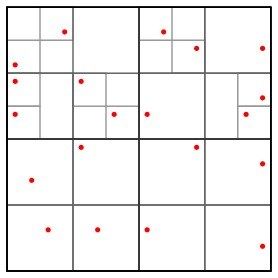
\includegraphics[scale=0.75]{fcarc-march2012-quadtree}
  
    \begin{itemize}
      \item Approximated TSP (PTAS) 
      \begin{itemize}
        \item Komplexität: $O(n {(log n)}^{O(c)})$
        \item Quadtree als Clustering-Methode
      \end{itemize}
    \end{itemize}
  \end{center}
\end{frame}

\section{Abschluss}

\begin{frame}
  \frametitle{Quad-/Octrees}
  \framesubtitle{Andere Anwendungen}
  \begin{itemize}
    \item Punktemenge (Alt. zu Punkteashverfahren wie z.B. Morton-Code)
    \item Nachbarsuche
    \item Frustum Culling
    \item Sparse data storage (Spreadsheets/Matrizen)
    \item Maximum disjoint sets
  \end{itemize}
\end{frame}

\begin{frame}
  \frametitle{Quad-/Octrees}
  \framesubtitle{Schlussfolie}
  \begin{center}
    Vielen Dank für die Aufmerksamkeit! \\
    \hfill\break
    Fragen?
  \end{center}
\end{frame}

\begin{frame}
  \frametitle{Quad-/Octrees}
  \framesubtitle{Literatur}
  \begin{itemize}
    \item Hanan, \emph{The Design and Analysis of Spatial Data Structures}, Addison-Wesley, Reading, MA, 1990, ISBN 0-201-50255-0.
    \item Berg, Kreveld, Overmans, Schwarzkopf, \emph{The Design and Analysis of Spatial Data Structures}, Addison-Wesley, Reading, MA, 1990, ISBN 0-201-50255-0.
    \item Austin, \emph{A (Very Short) Detour for the Traveling Salesman}, American Mathematical Society, 2012.
  \end{itemize}
\end{frame}

\end{document}
